\documentclass[12pt, fleqn]{report}

\usepackage{indentfirst}
\usepackage{graphicx}
\usepackage{fontspec}
\usepackage{geometry}
\usepackage{setspace}
\usepackage{caption}
\usepackage{float}
\usepackage{titlesec}
\usepackage{unicode-math}
\usepackage[none]{hyphenat}
\usepackage{titletoc}
\usepackage{tocloft}
\usepackage{xcolor}
\usepackage[colorlinks=true,citecolor=black,linkcolor=black]{hyperref}
\usepackage{amsmath}
\usepackage{changepage}
\usepackage{siunitx}


\geometry{
    a4paper,
    left=3.0cm,
    right=1.5cm,
    top=2.0cm,
    bottom=2.5cm
}

\setmainfont{DejaVu Serif}
\onehalfspacing
\floatplacement{figure}{H}

\setlength{\parskip}{10pt}
\setlength{\parindent}{1cm}

\newcommand{\titlespc}{\vspace{15pt}}

\titleformat{\chapter}[hang]
  {\normalfont\Large\bfseries}{Գլուխ \thechapter․}{10pt}{\raggedright\Large}

\titlespacing*{\chapter}{0pt}{-30pt}{10pt}

\titleformat{\section}[hang]
    {\normalfont\large\bfseries}{\thesection}{10pt}{\raggedright\large}
    \vspace{-20pt}

\titlespacing*{\section}{0pt}{0pt}{5pt}

\setmathfont{XITS Math}

\renewcommand{\cftchappresnum}{Chapter }
\renewcommand{\cftchapnumwidth}{6em}
\renewcommand{\cftchapaftersnum}{\hspace{1em}}
\renewcommand{\cftchapleader}{\cftdotfill{\cftdotsep}}

\hypersetup{
    colorlinks=true,
    linkcolor=black,
    urlcolor=blue,
    pdfborder={0 0 0},
}

\begin{document}

\emergencystretch 3cm

    \thispagestyle{empty}
    \begin{center}
        \fontseries{md}{
            \fontsize{16}{16}\selectfont ԵՐԵՎԱՆԻ ՊԵՏԱԿԱՆ ՀԱՄԱԼՍԱՐԱՆ
            \vspace{15pt} \\
            \fontsize{14}{14}\selectfont ՖԻԶԻԿԱՅԻ ԻՆՍՏԻՏՈՒՏ
            \vspace{80pt} \\
            \fontsize{18}{18}\selectfont Սիմոնյանց Դավիթ Վաչեի
            \vspace{50pt} \\
            \fontsize{30}{30}\selectfont ԱՎԱՐՏԱԿԱՆ ԱՇԽԱՏԱՆՔ
            \vspace{35pt} \\
            \fontsize{18}{18}\selectfont ԹԵՄԱ՝
            \vspace{15pt} \\
            
            \fontsize{14}{14}\selectfont Անտենաների թերությունների և ճառագայթվող էլեկտրամագնիսական դաշտի հետազոտումը ջերմաառաձգական օպտիկական ինդիկատորով մանրադիտակի օգնությամբ

            \vfill
            {\fontsize{13}{15}\selectfont ԵՐԵՎԱՆ 2023}
        }
    \end{center}

\newpage

\titlecontents{chapter}
  [0pt]
  {\addvspace{10pt}\bfseries}
  {\makebox[2.5em][l]{\textbf{Գլուխ~\thecontentslabel}.} \hspace{0.0em}}
  {}
  {\hfill\contentspage}
  
\renewcommand{\contentsname}{Բովանդակություն}

\tableofcontents

\newpage

\captionsetup[figure]{name=Նկ․}
\captionsetup{justification=raggedright, width=1.0\textwidth, font=small, format=hang}

\phantomsection
\section* {Ներածություն}
\addcontentsline{toc}{section}{Ներածություն}

Անտենաների գործունեությունը կարևոր դեր ունի ժամանակակից հեռահաղորդակցման բազմաթիվ ոլորտներում՝ անլար ցանցերից մինչև արբանյակային կապեր։ Էլեկտրամագնիսական ալիքների ճշգրիտ և էֆեկտիվ հաղորդումը կարևոր նշանակություն ունի անտենաների ճիշտ աշխատանքի համար։ Միևնույն ժամանակ անտենայում հայտնվող թերությունները կարող են բերել դրանց աշխատանքի սխալ կատարման և ազդանշանների կորուստի կամ աղավաղման, ինչի արդյունքում նվազում է անտենայի հաղորդակցման տիրույթը և հուսալիությունը։ Ուստի անտենաների ճառագայթած էլեկտրամագնիսական դաշտերի հետազոտումը և հնարավոր դեֆեկտեների հայտնաբերումը կարևոր նշանակություն ունի հեռահաղորդակցման ոլորտում։

Այս խնդրին և նմանատիպ այլ խնդիրներին լուծումներ են առաջարկվել հիմնված տարատեսակ ֆիզիկական երևույթների վրա։ Դրանցից օրինակ են սկանավորող ջերմային մանրադիտումը (Scanning thermal microscopy (SThM)), մերձադաշտային օպտիկական մանրադիտումը (Near-field scanning optical microscopy (NSOM)) կամ այլ սկանավորման տեխնիկայի վրա հիմնված լուծումներ։ Չնայած նրան, որ սկանավորման տեխնիկան ունի տասնյակ նանոմետրերի հասնող բարձր տարածական լուծունակություն \cite{yue2012nanoscalethermal}, նրա գործողության երկար ժամանակը իր գլխավոր թերություններից է և հնարավորություն չի թողնում կատարել ժամանակից կախված չափումներ։ Բացի դրանից, սկանավորման տեխնիկան պահանջում է թանկարժեք և դժվար հասանելի նյութեր և սարքավորումներ և չափումների խիստ պայմաններ։ Մասնավորապես SThM֊ը նաև պահանջում է հպում չափվող նմուշի հետ, ինչը բերում է նմուշի ջերմահաղորդականության հետևանքով ջերմային բաշխվածության չափման սխալանքների։

Վերջին տարիներում առաջացել և զարգացել է ջերմաառաձգական օպտիկական ինդիկատորով մանրադիտակի (ՋԱՕԻՄ) վրա հիմնված, տարբեր նյութերում և սարքերում ջերմային և մեխանիկական հատկությունների հետազոտումը՝  բարձր զգայունությամբ և տարածական լուծունակությամբ։ ՋԱՕԻՄ֊ը սարք է, որը հնարավորություն է տալիս հետազոտել էլեկտրամագնիսական կամ ջերմային ճառագայթման աղբյուր հանդիսացող սարքերից ճառագայթվող էլեկտրամագնիսական դաշտերը կամ ջերմային բաշխվածությունները։ Այն օգտագործվում է բազմաթիվ սարքերի, օրինակ՝ էլեկտրոսխեմաների, հիշասարքերի, բարձր կամ ցածր հաճախային ֆիլտրերի ճառագայթման հետազոտման, այդ սարքերում  ճառագայթման վրա ազդեցություն թողած թերությունների հայտնաբերման համար։

ՋԱՕԻՄ֊ի աշխատանքի սկզբունքը կայանում է նրանում, որ նրա ինդիկատորը կլանում է էլեկետրամագնիսական կամ ջերմային ճառագայթումը, վերածելով այն ջերմության։ Ինդիկատորում առաջացած ջերմությունը նրա մեջ առաջացնում է ջերմամեխանիկական լարումներ, որոնց բաշխվածությունները չափվում են ֆոտոէլաստիկ երևույթների վրա հիմնված եղանակով։ Չափումներից վերականգնվում է ինդիկատորում ջերմային բաշխվածությունը։ Համապատասխան հատկություններով ինդիկատոր ընտրելու դեպքում, եթե ջերմության պատճառը էլեկտրամագնիսական դաշտն էր, ապա վերականգնված ջերմային բաշխվածությունը նկարագրում է ինդիկատորում առաջացած էլեկտրամագնիսական դաշտը։

ՋԱՕԻՄ֊ի միջոցով չափված ինտենսիվության կամ ջերմության բաշխվածությունը ունենում է բավականին բարձր տարածական լուծունակություն և ջերմային զգայունություն։ Ի տարբերություն սկանավորման տեխնիկայի, ՋԱՕԻՄ֊ի համար պահանջվող նյութերն ու սարքերը օրինակ՝ սովորական ապակին, CCD (charge-coupled device) տեսախցիկը կամ բևեռացրած լույսի միկրոսկոպը, հեշտ հասանելի են և ոչ թանկ։ Ինչպես նաև ՋԱՕԻՄ֊ի արագ աշխատանուկաթյունը հնարավորություն է տալիս ժամանակից կախված չափումներ իրականացնել։ ՋԱՕԻՄ֊ի այս հատկությունները, ինչպես նաև չափումների պարզությունը նրան դարձնում են անտենաների ճառագայթվող էլեկտրամագնիսական դաշտերի հետազոտման համար հարմար և գրավիչ միջոց։

Այս աշխատանքի նպատակն է ցույց տալ, թե ինչպես է հնարավոր ՋԱՕԻՄ֊ի օգնությամբ բարձր լուծունակությամբ և ջերմային զգայունությամբ արտապատկերել և ուսումնասիրել ալիքատարային անտենայի ճառագայթած էլեկտրամագնիսական դաշտը։ Ներկայացվելու է ՋԱՕԻՄ համակարգի աշխատանքի սկզբունքը և այն օգտագործող փորձի նկարագրությունը։ Վերջում ներկայացվելու են փորձի արդյունքները և քննարկումները։

Անտենայի ճառագայթած էլեկտրամագնիսական դաշտի ուսումնասիրությունը ջերմաառաձգական օպտիկական ինդիկատորով մանրադիտակի օգնությամբ հնարավորություն կարող է ընձեռնել բարելավել անտենաների աշխատունակությունը և հուսալիությունը։ Այս ուսումնասիրությունը կարող է բերել բարելավված անտենաների նախագծերի մշակման և գոյություն ունեցող անտենաների բարելավման։

\newpage

\renewcommand{\thesection}{\arabic{section}}

\section{Փորձի նկարագրությունը}
\subsection{ՋԱՕԻՄ֊ի կառուցվածքը}

Նկ․ \ref{fig:TEOIM-scheme}֊ում պատկերված է ՋԱՕԻՄ֊ի փորձարարական սխեման \cite{arakelyan2016teoim}։ Հետազոտվող սարքի վրա տեղադրված է օպտիկական ինդիկատոր, որը իրենից ներկայացնում է ջերմային կամ էլեկտրամագնիսական ճառագայթում կլանող նանոմետրական շերտով ապակի։ Սովորական LED֊ից ինդիկատորի վրա ընկած է լույս, որը սկզբից անցնում է հարթ բևեռացուցչով, այնուհետև անցնում է հեղուկ֊բյուրեղային մոդուլյատորով և ձեռք բերում շրջանային բևեռացում։ Շրջանային բևեռացած լույսն ընկնելով ինդիկատորի վրա, կլանիչ շերտից անդրադառնալով անցնում է վերլուծիչով և նրա բևեռականության փոփոխությունները գրանցվում են CCD տեսախցիկով։

\begin{figure}
    \centering
    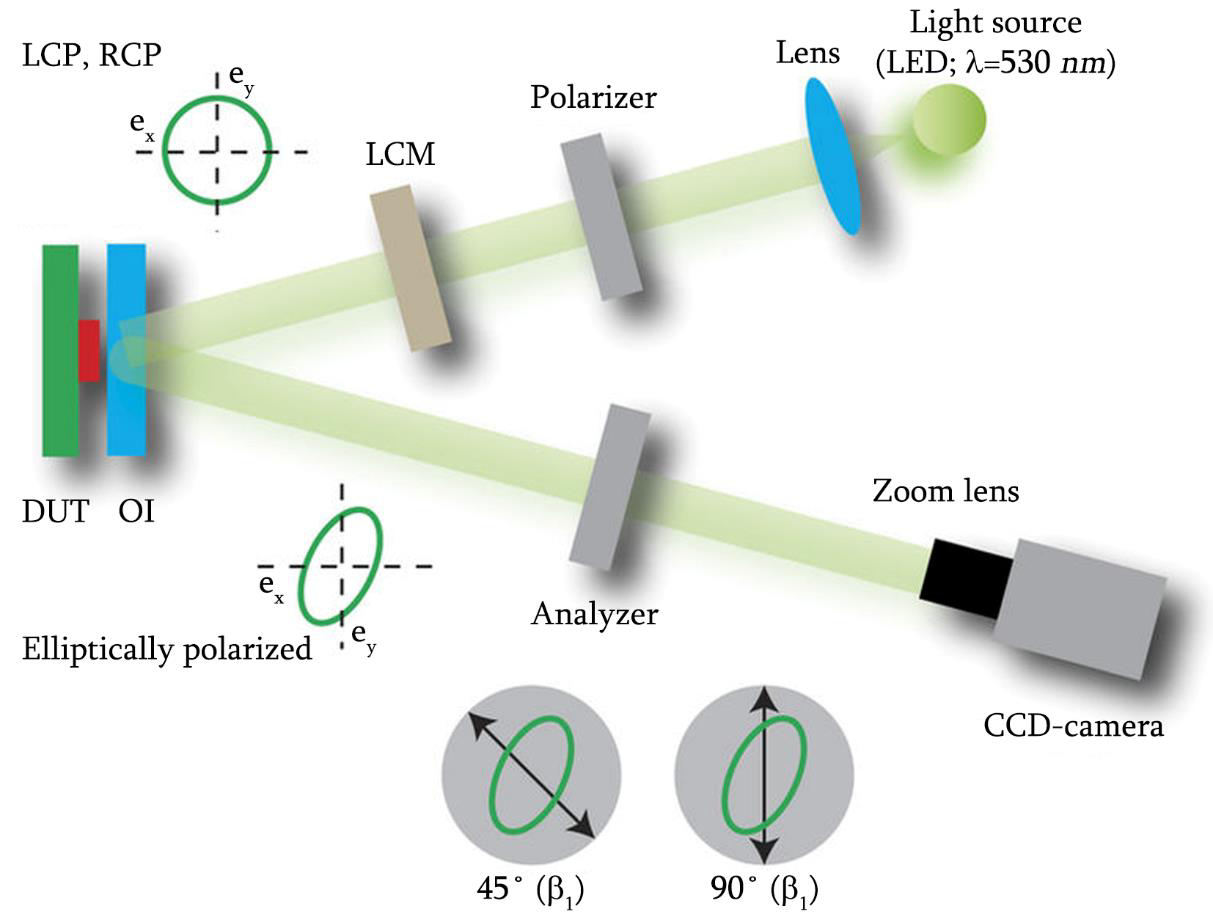
\includegraphics[width=1.0\textwidth]{data/TEOIM/0.jpg}
    \caption{Փորձի սկզբունքային սխեման}
    \label{fig:TEOIM-scheme}
\end{figure}
Ինչպես պատկերված է նկ․ \ref{fig:TEOIM-photoelasticity}֊ում, կախված շերտի նյութի հատկություններից, ինդիկատորը կարող է կլանել ջերմային ճառագայթում կամ իր ներսում էլեկտրամագնիսական ճառագայթումը կկրի ջերմային կորուստներ։ Կլանող շերտում առաջացած ջերմությունը տարածվում է իր ամբողջ ջերմաէլաստիկ միջավայրով և նրանում առաջացնում է ջերմամեխանիկական լարումներ։ Ջերմամեխանիկական լարումների պատճառով ինդիկատորի վրա ընկած շրջանային բևեռացված լույսը, կախված իր դիրքում լարվածության առանցքի կողմնորոշումից, կլանող շերտի միջավայրում կփոխի իր բևեռացվածությունը էլիպտիկի։ Այս երևույթը հայտնի է որպես ֆոտոէլաստիկ երևույթ։ Այնուհետև \SI{0}{\degree} և \SI{45}{\degree} աստիճան կողմնորոշմամբ վերլուծիչից անցած լույսի ինտենսիվությամբ կարելի է չափել հետազոտվող սարքի պատճառով օպտիկական ինդիկատորում առաջացած գծային երկբեկման փոփոխությունը։

\begin{figure}
    \centering
    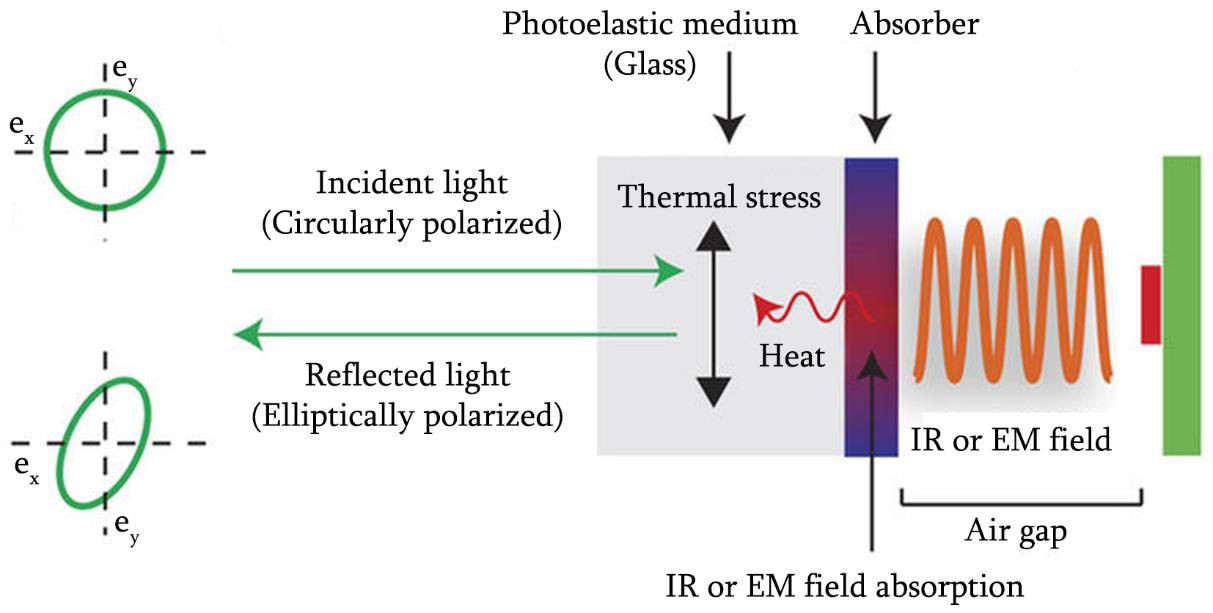
\includegraphics[width=1.0\textwidth]{data/TEOIM/1.jpg}
    \caption{Ինդիկատորում կլավնած ջերմային կամ էլեկտրամագնիսական ճառագայթումից առաջացած ջերմամեխանիկական լարումների պատճառով շրջանային բևեռացրած լույսի վերափոխումը էլիպտիկ բևեռացվածի։}
    \label{fig:TEOIM-photoelasticity}
\end{figure}

\subsection{Ջերմային բաշխվածության արտապատկերումը}
Գտնենք ջերմամեխանիկական լարման կապը նորմալ և սահքի լարումներով պայմանավորված գծային երկբեկման բաշխվածությունների հետ։ Նկ․ \ref{fig:TEOIM-optical-components}֊ում օպտիկական սարքերից յուրաքանչյուրի համար Ջոնի մատրիցը տրվում է հետևյալ կերպ՝
\begin{flalign}
J_p &= \begin{pmatrix}
            1 & 0 \\
            0 & 0
        \end{pmatrix}, J_{LCM} = \frac{1}{2} \begin{pmatrix}
            e^{i \frac{\delta}{2}} + e^{-i \frac{\delta}{2}} & e^{i \frac{\delta}{2}} - e^{-i \frac{\delta}{2}} \\
            e^{i \frac{\delta}{2}} - e^{-i \frac{\delta}{2}} & e^{i \frac{\delta}{2}} + e^{-i \frac{\delta}{2}}
        \end{pmatrix}, J_A = \begin{pmatrix}
            \cos^2{\phi} & \cos{\phi}\sin{\phi} \\
            \cos{\phi}\sin{\phi} & \sin^2{\phi}
        \end{pmatrix},
        \end{flalign}
որտեղ՝ $\delta$֊ն հեղուկ֊բյուրեղային մոդուլյատորի գծային երկբեկումն է, իսկ $\phi$֊ն վերլուծող բևեռացուցիչի և $x$ առանցքի հետ կազմած անկյունը։ Գծային և շրջանային փոխադարձելիության և շրջանային երկբեկման պայմաններում ինդիկատոորի համար Ջոնի մատրիցը կընդունի հետևյալ տեսքը  \cite{xie1990picosecond}՝
\begin{flalign}
J_s &= \begin{pmatrix}
    e^{i\beta}\cos^2{\theta} + e^{-i\beta}\sin^2(\theta) & (e^{i\beta} - e^{-i\beta})\cos{\theta}\sin{\theta} \\
    (e^{i\beta} - e^{-i\beta})\cos{\theta}\sin{\theta} &
    e^{i\beta}\cos^2{\theta} + e^{-i\beta}\sin^2(\theta)
\end{pmatrix}, &&
\end{flalign}
որտեղ՝ $\beta$֊ն ինդիկատորում ջերմամեխանիկական լարումներից առաջացած գծային երկբեկումն է, իսկ $\theta$֊ն՝ լարման սկզբունքային առանցքի և վերլուծող բևեռացուցիչի կազմած անկյունը։

\begin{figure}
    \centering
    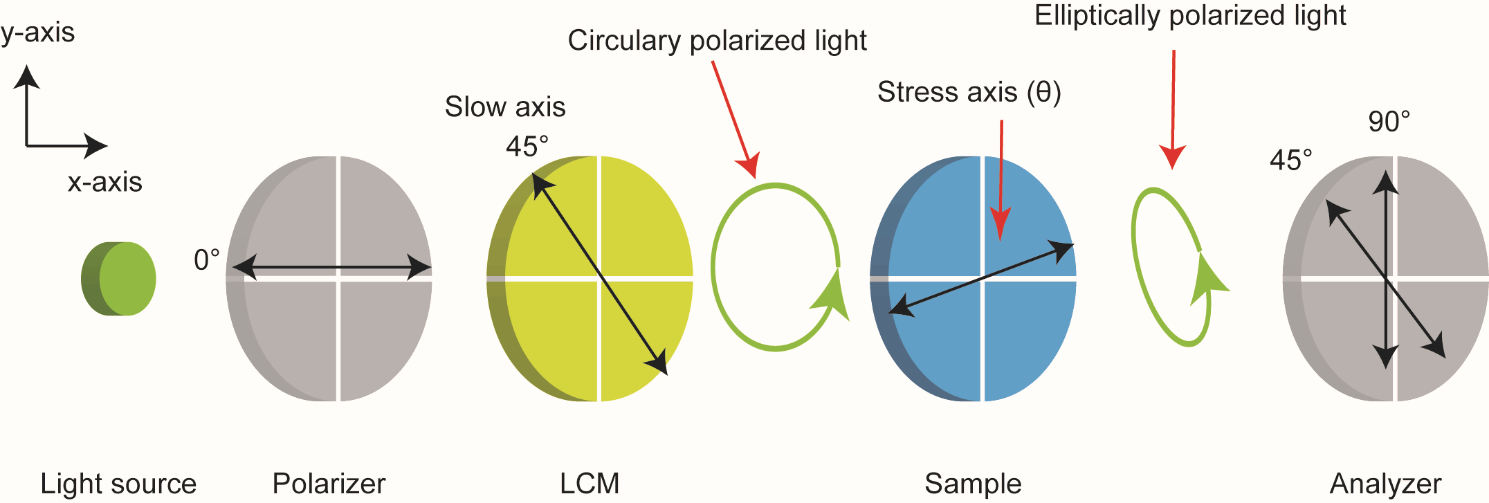
\includegraphics[width=1.0\textwidth]{data/TEOIM/2.jpg}
    \caption{Փորձում օգտագործվող օպտիկական բաղադրիչների անկյունային կողմնորոշումները։}
    \label{fig:TEOIM-optical-components}
\end{figure}
CCD տեսախցիկին ընկնող լույսի ինտենսիվությունը կորոշվի հետևյալ բանաձևով՝
\begin{flalign}
I &= \frac{E_i^2}{4}(|A|^2 \cos^2{\phi} + |B|^2 \sin^2{\phi} + (A^*B + AB^*)\cos{\phi}\sin{\phi}), &&
\label{eq:analyzed_light_intensity}
\end{flalign}
որտեղ՝ $E_i$֊ն ընկնող լույսի էլեկտրական դաշտի լայնույթն է, իսկ $A$֊ն ու $B$֊ն ներկայացվում են հետևյալ կերպ՝
\begin{flalign}
A &= j_1 \delta_+ + j_2 \delta_-, \hspace{0.5cm} B = j_2 \delta_+ + j_1 \delta_-, \\
j_1 &= e^{i\beta} \cos^2{\phi} + e^{-i\beta} \sin^2{\phi}, \hspace{0.5cm} j_2 = (e^{i\beta} - e^{-i\beta}) \cos{\phi} \sin{\phi}, \\
\delta_+ &= e^{i\frac{\delta}{2}} + e^{-i\frac{\delta}{2}}, \hspace{0.5cm} \delta_- = e^{i\frac{\delta}{2}} - e^{-i\frac{\delta}{2}},
\label{eq:AB_js_deltas}
\end{flalign}
Հաշվի առնելով \eqref{eq:analyzed_light_intensity}-\eqref{eq:AB_js_deltas} բանաձևերը և անկման լույսի շրջանային բևեռացվածությունը, CCD տեսախցիկին հասնող լույսի ինտենսիվության համար ունենք՝
\begin{flalign}
I_{\phi=\pi/2, \delta=-\pi/2} &= \frac{E_i^2}{2}(1 - \sin{2\beta}\sin{2\theta}), \hspace{0.5cm} I_{\phi=\pi/2, \delta=\pi/2} = \frac{E_i^2}{2}(1 + \sin{2\beta}\sin{2\theta}), \\
I_{\phi=\pi/4, \delta=-\pi/2} &= \frac{E_i^2}{2}(1 - \sin{2\beta}\cos{2\theta}), \hspace{0.5cm} I_{\phi=\pi/4, \delta=\pi/2} = \frac{E_i^2}{2}(1 + \sin{2\beta}\cos{2\theta}),
\end{flalign}
$\beta$֊ի փոքր անկյունների դեպքում՝
\begin{flalign}
\hspace{-1cm}\beta_1 &= \frac{1}{2} \frac{I_{\phi=\pi/4, \delta=\pi/2} - I_{\phi=\pi/4, \delta=-\pi/2}}{I_{\phi=\pi/4, \delta=\pi/2} + I_{\phi=\pi/4, \delta=-\pi/2}} \approx \beta \cos{2\theta},
\beta_2 = \frac{1}{2} \frac{I_{\phi=\pi/2, \delta=\pi/2} - I_{\phi=\pi/2, \delta=-\pi/2}}{I_{\phi=\pi/2, \delta=\pi/2} + I_{\phi=\pi/2, \delta=-\pi/2}} \approx \beta \sin{2\theta}
\label{eq:linear-birefringence}
\end{flalign}
Ենթադրվում է, որ ջերմամեխանիկական լարումները բնութագրվում են երկչափ թենզորով, քանի որ ինդիկատորի նանոմետրական շերտի չափը երրորդ չափողականությամբ անհամեմատ փոքր է մյուս երկու ուղղությամբ չափումներից։ Մեխանիկական թենզորի համար ունենք՝
\begin{flalign}
    \sigma &= \begin{pmatrix}
        \sigma_{xx} & \sigma_{xy} \\
        \sigma_{yx} & \sigma_{yy}
    \end{pmatrix} = \begin{pmatrix}
        \sigma_1 \cos^2{\theta} + \sigma_2 \sin^2{\theta} & (\sigma_1 - \sigma_2) \cos{\theta} \sin{\theta} \\
    (\sigma_1 - \sigma_2) \cos{\theta} \sin{\theta} & \sigma_1 \cos^2{\theta} + \sigma_2 \sin^2{\theta}
    \end{pmatrix}, &&
    \label{eq:mechanical-tensor}
\end{flalign}
որտեղ՝ $\sigma_1$֊ը և $\sigma_2$֊ը մեխինակական լարումների սկզբունքային առանցքներն են։ \eqref{eq:linear-birefringence} և \eqref{eq:mechanical-tensor} բանաձևերից կստանանք կապը գծային երկբեկման և մեխանիկական լարման միջև՝
\begin{flalign}
    \beta_1 &= \frac{2\pi dS}{\lambda}(\sigma_{xx} - \sigma_{yy}), \hspace{0.5cm} \beta_2 = \frac{2\pi dS}{\lambda}2\sigma_{xy}, &&
\end{flalign}
որտեղ՝ $S$֊ը լարման օպտիկական հաստատունն է, $\lambda$֊ն ընկնող լույսի ալիքի երկարությունն է, իսկ $d$֊ն ինդիկատորի հաստությունն է։

Գտնենք կապը ջերմային բաշխման և մեխանիկական լարման միջև։ Հարթությամբ ազդող ուժերի դեպքում ջերմային լարումները կարելի է ներկայացնել հետևյալ բանաձևերով \cite{barron2011thermalstress}՝
\begin{flalign}
    \sigma_{xx} &= \frac{\partial^2 \varPhi} {\partial y^2} + CT,
    \hspace{0.5cm}
    \sigma_{yy} = \frac{\partial^2 \varPhi}{\partial x^2} + CT,
    \hspace{0.5cm}
    \sigma_{xy} = -\frac{\partial^2 \varPhi} {\partial x \partial y},
    \hspace{0.1cm}
    C = \frac{\alpha E}{1 - 2 \nu},
    \label{eq:thermal-stress}
\end{flalign}
որտեղ  $T$֊ն ջերմաստիճանային բաշխվածությունն է, $\alpha$֊ն ջերմային ընդարձակման գործակիցն է, $\nu$֊ն Պուասոնի գործակիցն է, $E$֊ն Յունգի մոդուլն է, իսկ $\varPhi$֊ն լարման ֆունկցիան է և բավարարում է հետևյալ հավասարմանը՝
\begin{flalign}
    \nabla^4 \varPhi &= - \frac{\alpha E}{1 - \nu} \nabla^2 T,
\end{flalign}
\eqref{eq:thermal-stress}֊ից կստանանք՝
\begin{flalign}
    -\frac{\partial(\sigma_{xx} - \sigma_{yy})}{\partial x} - 2 \frac{\partial \sigma_{xy}}{\partial y} &= \frac{\partial (\nabla^2\varPhi)}{\partial x},
    \hspace{0.5cm}
    -\frac{\partial(\sigma_{xx} - \sigma_{yy})}{\partial y} - 2 \frac{\partial \sigma_{xy}}{\partial x} = \frac{\partial (\nabla^2\varPhi)}{\partial y},
\end{flalign}
որից կստանանք կապը լարման ֆունկցիայի և գծային երկբեկման միջև՝
\begin{flalign}
    \frac{\partial (\nabla^2 \varPhi)}{\partial x} &= -\frac{\lambda} {2\pi dS} \left( \frac{\partial \beta_1}{\partial x} + \frac{\partial \beta_2}{\partial y} \right),
    \hspace{0.5cm}
    \frac{\partial (\nabla^2 \varPhi)}{\partial y} = -\frac{\lambda} {2\pi dS} \left( \frac{\partial \beta_1}{\partial y} - \frac{\partial \beta_2}{\partial x} \right), &&
    \label{eq:stress_function_vs_linear_birefringence}
\end{flalign}
Ջերմահաղորդականության հավասարումից, ստացիոնար ջերմային աղբյուրի դեպքում նրա բաշխվածությունը որոշվում է հետևյալ բանաձևով՝
\begin{flalign}
    q = -\frac{(1 - \nu) k}{\alpha E} \left( \frac{\partial^2(\nabla^2 \varPhi)}{\partial x^2} + \frac{\partial^2(\nabla^2 \varPhi)}{\partial y^2} \right), \hspace{0.5cm} q = k\nabla^2T,
    \label{eq:thermal_conductivity}
\end{flalign}
որտեղ $q$֊ն ջերմային բաշխվածությունն է, իսկ $k$֊ն ինդիկատորի էֆեկտիվ ջերմահաղորդականությունը։ \eqref{eq:stress_function_vs_linear_birefringence}֊ից և \eqref{eq:thermal_conductivity}֊ից կստանանք կապը ջերմային բաշխվածության և գծային երկբեկման միջև՝
\begin{flalign}
    q &= \frac {\lambda}{2\pi dS} \frac{1 - \nu}{\alpha Ek}
    \left( 2 \frac{\partial^2 \beta_2}{\partial x \partial y} +  \frac{\partial^2 \beta_1}{\partial x^2} - \frac{\partial^2\beta_1}{\partial y^2} \right): &&
\label{eq:TD_vs_LB}
\end{flalign}
\subsection{Էլեկտրամագնիսական դաշտի կորուստները}
Բարձր ջերմահաղորդականությամբ օժտված ինդիկատորը լավ է կլանում իր մեջ ջերմային ճառագայթումը և ստացված գծային երկբեկմամբ հնարավոր է լինում արտապատկերել ջերմային ճառագայթումը ինդիկատորի մեջ։ Սակայն ինդիկատորի նանոմետրական շերտի համապատասխան հատկություններով նյութ ընտրելու դեպքում ինդիկատորում էլեկտրամագնիսական ճառագայթումը կկրի ջերմային կորուստներ, որից առաջացած ջերմային բաշխվածության արտապատկերումը կնկարագրի ինդիկատորում էլեկտրամագնիսական դաշտի ինտենսիվության բաշխվածությունը։
Համարելով ինդիկատորի ապակու ջերմահաղորդականությունը համասեռ, էլեկտրամագնիսական կորուստներով ինդիկատորի ապակյա տակդիրում ջերմաստիճանի փոփոխությունը կնկարագրվի հետևյալ բանաձևով՝
\begin{flalign}
    \rho C_p \frac{\partial T}{\partial t} - \nabla (k\nabla T) &= q,
\end{flalign}
որտեղ՝ $\rho$֊ն ապակյա տակդիրի խտությունն է, $k$֊ն՝ ջերմահաղորդականությունը, $C_p$֊ն՝ ջերմունակությունը, իսկ $q$֊ն էլեկտրամագնիսական կորուստներով նյութում ջերմության բաշխվածությունն է։ Ստացիոնար վիճակում հավասարումը պարզեցվում է՝
\begin{flalign}
    -k \nabla^2 T &= q: &&
\end{flalign}
Կախված ինդիկատորի նանոմետրական շերտի նյութից, էլեկտրական կամ մագնիսական դաշտը ինդիկատորում կարող է կրել ջերմային կորուստներ։ Եթե շերտը դիէլեկտրիկ կորուստներով նյութ է, ապա էլեկտրական դաշտը կրում է ջերմային կորուստներ։ Առաջացած ջերմային էներգիայի խտությունը կորոշվի հետևյալ բանաձևով՝
\begin{flalign}
    q &= \frac{\omega}{2} \varepsilon'' |E|^2,
\end{flalign}
որտեղ՝ $\omega$֊ն էլեկտրամագնիսական դաշտի հաճախությունն է, իսկ $\varepsilon''$֊ն կորուստներով շերտի դիէլեկտրիկ թափանցելիության կեղծ մասն է, իսկ $E$֊ն՝ էլեկտրական դաշտի լայնույթը։

Եթե նանոմետրական շերտը բարձր հաղորդականությամբ նյութ է, ապա մագնիսական դաշտը նրանում մակածում է մրրկային հոսանքներ, որոնք կրում են ջերմային կորուստներ։ Առաջացած ջերմային էներգիայի խտությունը կորոշվի  հետևյալ բանաձևով՝
\begin{flalign}
    q &= \frac{P_{av}}{V} = \frac{R_s}{2t}|H_t|^2, \\
    \label{eq:TD_vs_Ht}
    P_{av} &= \int\frac{R_s}{2}|H_t|^2dS, \\
    R_s &= \sqrt{\frac{\omega \mu}{2\sigma}} = \frac{1}{\sigma \delta_s},
\end{flalign}
որտեղ $P_{av}$֊ն հաղորդիչ շերտի կլանած էլեկտրամագնիսական հզորությունն է, $R_s$֊ը և $\delta_s$֊ը համապատասխանաբար շերտի մակերևույթային դիմադրությունն է և սկին շերտի հաստությունը, $H_t$֊ն հաղորդիչ շերտի նկատմամբ մագնիսական դաշտի տանգենցիալ բաղադրիչն է, իսկ $t$֊ն շերտի հաստությունն է։

\subsection{Տվյալների հավաքագրումը և վերամշակումը}
\begin{figure}
    \centering
    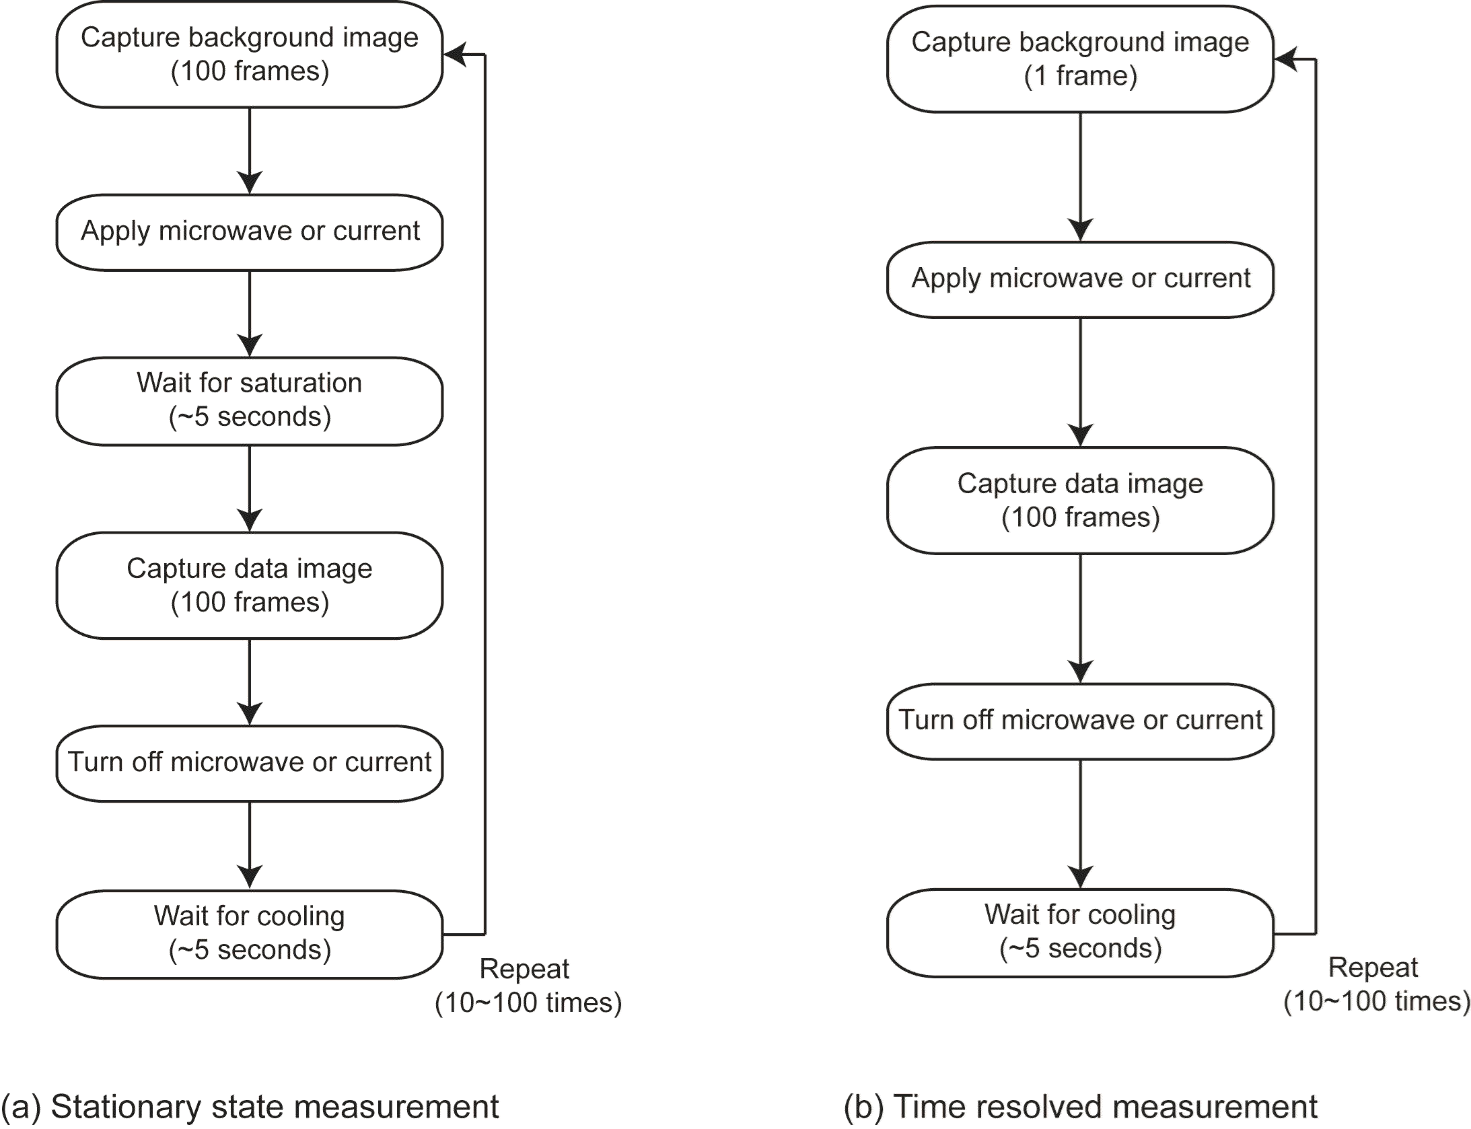
\includegraphics[width=1.0\textwidth]{data/TEOIM/3.png}
    \caption{Տվյալների հավաքագրման քայլերի հերթականությունը (a) ստատիկ չափումների և (b) ժամանակից կախված չափումների դեպքում։}
    \label{fig:data-collection-steps}
\end{figure}
CCD տեսախցիկով արված պատկերները հավաքագրվում են և վերամշակվում։ Նկ․ \ref{fig:data-collection-steps}֊ում ցույց է տրված ստատիկ և ժամանակից կախված չափումների դեպքում տվյալների հավաքագրման քայլերը։ Ստատիկ չափումներում սկզբից CCD տեսախցիկով վերցվում են «հենքային» (background) տվյալների պատկերները և միջինացվում, այնուհետև միացվում է ջերմային կամ էլեկտրամագնիսական ճառագայթման աղբյուրը և մոտ 5 վրկ հագեցումից հետո, երբ ինդիկատորում հաստատվում է որոշակի ջերմային բաշխում, վերցվում և միջինացվում են «ինֆորմատիվ» (data) տվյալների պատկերները։ Ճառագայթման աղբյուրը անջատվում է և ինդիկատորը կրկին 5 վրկ հագենում է, որից հետո կատարվում է նույն փորձը 10-100 անգամ։ Ժամանակից կախված չափումների դեպքում «հենքային» պատկերը վերցվում է մեկ անգամ, այնուհետև ճառագայթման աղբյուրը միացնելուց հետո որոշակի ժամանակի ընթացքում վերցվում են «ինֆորմատիվ» պատկերները, որից հետո աղբյուրն անջատվում է և հագենում։ Նույն փորձը կրկնվում է 10֊100 անգամ։ Ընդհանուր առմամբ ստանում ենք 1000֊10000 միջինացվող կադր։
\begin{figure}
    \centering
    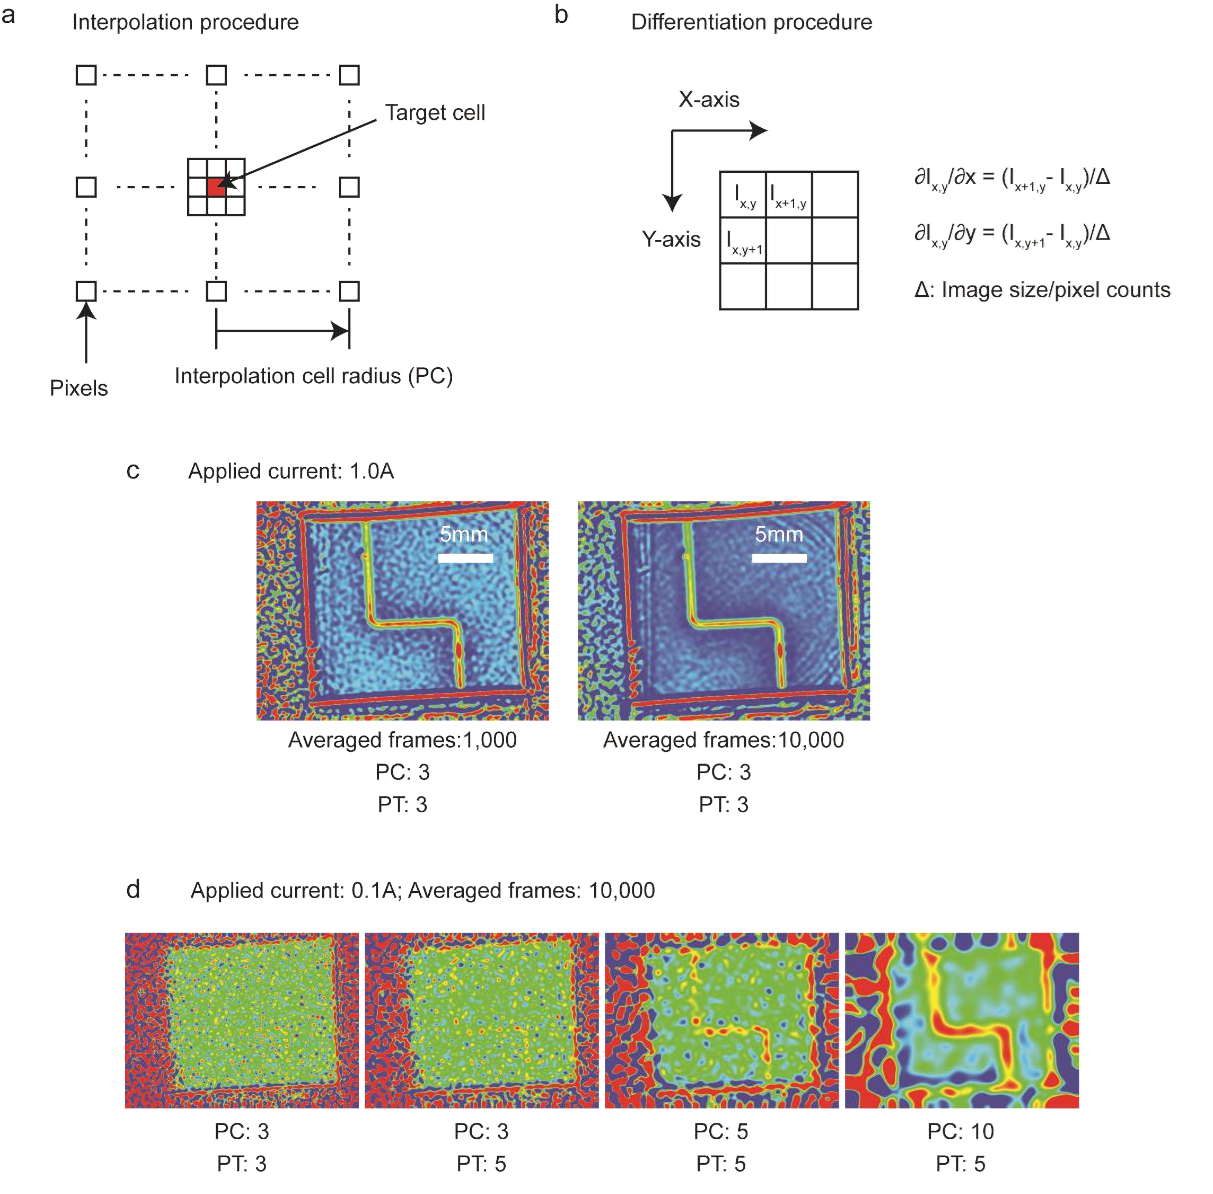
\includegraphics[width=1.0\textwidth]{data/TEOIM/4.png}
    \caption{(a) Պատկերի հարթեցման պրոցեսը։ (b) Պատկերի դիֆերենցման պրոցեսը։ (c) Հաշվարկված ջերմային բաշխվածությունը 1000 և 10000 կադրերի միջինացմամբ: (d) Հաշվարկված ջերմային բաշխվածությունը տարբեր չափերով «շարժվող բջիջի» տարբեր քանակի հարթեցումներից հետո։}
    \label{fig:frame-interp}
\end{figure}
Միջինացումից բացի պատկերները նաև հարթեցվում են, ինչպես ցույց է տրված նկ․ \ref{fig:frame-interp} (a)֊ում։ Հարթեցումը տեղի է ունենում «շարժվող բջիջի» միջոցով, որում բջիջի տակ եղած պատկերի պիկսելների ինտենսիվությունները միջինացվում են։ Այնուհետև պատկերները դիֆերենցվում են ըստ հորիզոնական և ուղղահայաց ուղղություններով հարևան պիկսելների ինտենսիվությունների տարբերության (b): Նկ․ \ref{fig:frame-interp}֊ի (c)֊ում և (d)֊ում ցույց են տրված տարբեր քանակի կադրերի միջինացումներից և տարբեր չափերի «շարժվող բջիջներով», տարբեր քանակի հարթեցումներից հետո ջերմային աղբյուրների հաշվարկված պատկերները։

\subsection{Ալիքատարային անտենայի հետազոտումը}
\begin{figure}
    \centering
    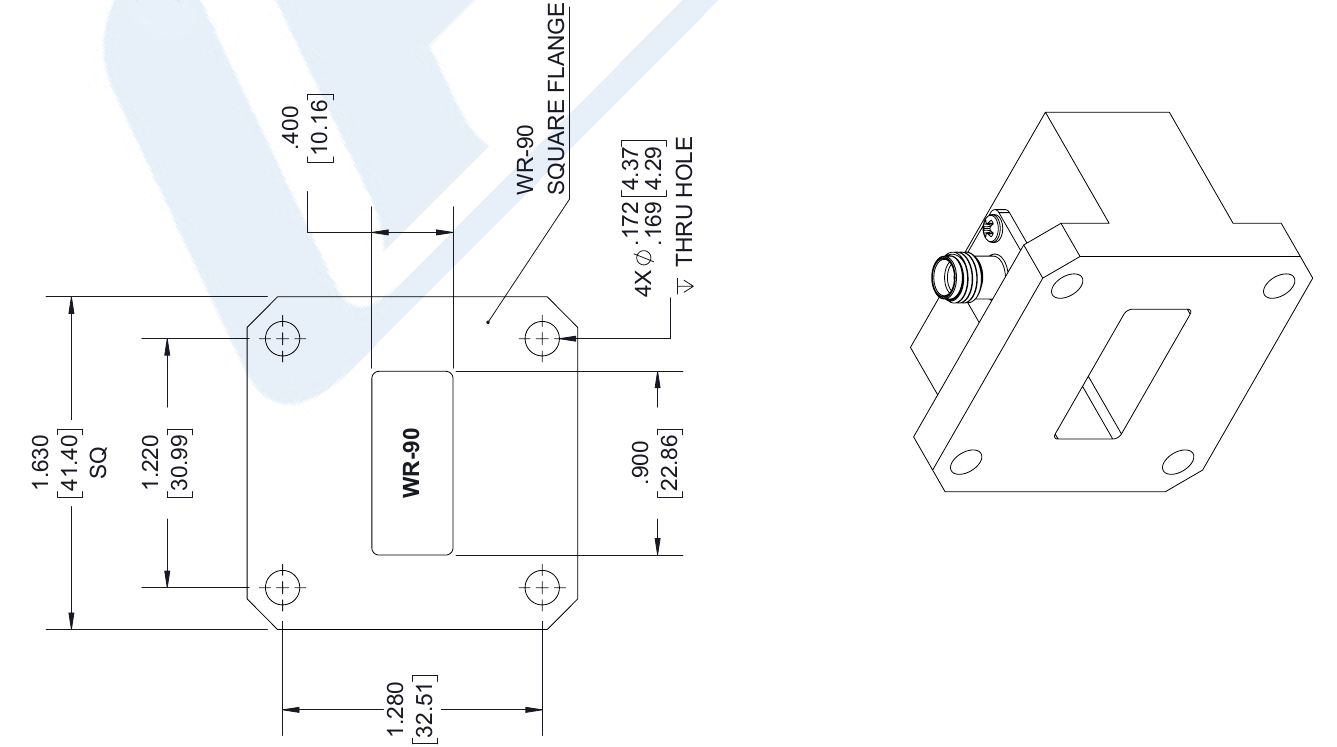
\includegraphics[width=1.0\textwidth]{data/waveguide/waveguide-scheme.png}
    \caption{PE9804 WR-90 ալիքատարի սխեմատիկ պատկերը}
    \label{fig:waveguide-scheme}
\end{figure}
ՋԱՕԻՄ֊ի միջոցով հետազոտվել է ալիքատարային անտենայի էլեկտրամագնիսական ճառագայթումը։ Օգտագործվել է PE9804 WR-90 մոդելի ուղղանկյուն ալիքատարը, որն էլ հենց օգտագործվել է որպես անտենա։ Նկ․ \ref{fig:waveguide-scheme}֊ում ցույց է տրված ալիքատարի սխեմատիկ պատկերը։ Այն ալյումինից պատրաստված ալիքատար է, որը նախագծված է անցկացնել [8.2֊12.4] ԳՀց հաճախային տիրույթում էլեկտրամագնիսական ալիքներ։ Նկ․ \ref{fig:waveguide-return-loss}֊ում կապույտ գրաֆիկը ցույց է տալիս նրա միջին մարման գործակիցը [8.2-12.4] ԳՀց հաճախային տիրույթում։ Կարմիր գրաֆիկը ցույց է տալիս նրա առավելագույն մարման գործակիցը։ Ուղղանկյուն ալիքատարը ունի 22.86 մմ լայնությամբ և 10.16 մմ բարձրությամբ ուղղանկյուն կտրվածք։ Այն տեղադրված է եղել օպտիկական ինդիկատորին հանդիպակաց՝ 5 մմ հեռավորության վրա։
\begin{figure}
    \centering
    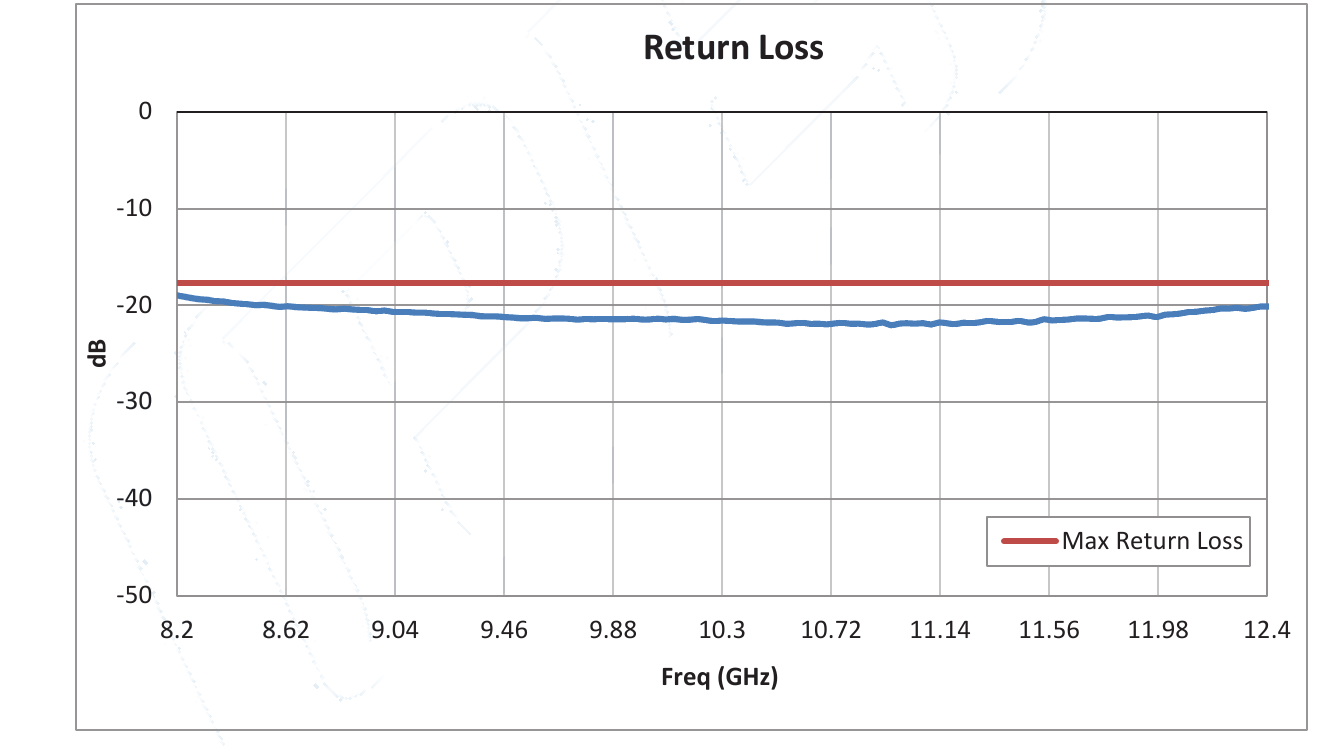
\includegraphics[width=1.0\textwidth]{data/waveguide/return-loss.png}
    \caption{PE9804 WR-90 ալիքատարի աշխատանքի տիրույթում հաճախությունից կախված մարման գործակիցը։}
    \label{fig:waveguide-return-loss}
\end{figure}
Որպես օպտիկական ինդիկատոր օգտագործվել է ինդիում֊անագի բարակ օքսիդային թաղանթով ապակին (ITO Glass): Ինդիում֊անագի օքսիդը թափանցիկ հաղորդիչ օքսիդ է, որն իրենից ներկայացնում է ինդիումի օքսիդի (In$_2$O$_3$) և անագի օքսիդի (SnO$_2$) պինդ լուծույթ։ Այն n տիպի կիսահաղորդիչ է շուրջ 4 ԷՎ արգելված գոտով։ ITO֊ն օժտված է բարձր հաղորդականությամբ (մոտ 10$^6$ Սմ/մ) և մեծ թափանցիկությամբ (90.2\%) \cite{chen2013itofabcrication}։ ITO֊ն օգտագործվում է տարբեր էլեկտրոնային սարքերում, օրինակ՝ սենսորային էկրաններում կամ արևային մարտկոցներում։ Ինդիում֊անագի օքսիդի բարակ թաղանթը հարթության վրա նստեցվում է հիմնականում ֆիզիկական գոլորշիների նստեցման (physical vapor deposition (PVD)) եղանակով։ Ինդիումի բարձր գնի և սահմանափակ քանակի, ինչպես նաև վակուում պահանջող թաղանթի նստեցման եղանակի բարձր գնի պատճառով ITO֊ի պատրաստման այլ եղանակների և ITO֊ին փոխարինող, թափանցիկ հաղորդիչ այլ նյութերի, օրինակ՝ գրաֆենի, ածխածնային նանոխողովակների, հաղորդիչ պոլիմերների ուսումնասիրություններ են կատարվել։

Ինդիկատորի ապակու վրա պատված ITO թաղանթի հաստությունը 100 նմ էր։  Ինչպես նշվեց, այսպիսի թաղանթով ինդիկատորը ունի բարձր հաղորդականություն, այսինքն նրանում, ինչպես հայտնի է, մագնիսական դաշտը մակածում է մրրկային հոսանքներ, որոնք նյութի դիմադրության պատճառով կրում են ջերմային կորուստներ։ Այսինքն չափվելու է ալիքատարի ճառագայթած  էլեկտրամագնիսական դաշտի հենց մագնիսական բաղադրիչը։

Փորձը բաժանված էր երեք մասի, փորձի յուրաքանչյուր մասում գեներացվել են որոշակի հզորության էլեկտրամագնիսական ալիքներ, որոնք անցկացվել են ուղղանկյուն ալիքատարով։ Փորձի առաջին մասում գեներացվել են 0 dBm, երկրորդում՝ 3 dBm, իսկ երրորդում՝ 6 dBm հզորությամբ էլեկտրամագնիսական ալիքներ։ Փորձի յուրաքանչյուր մասում հերթով ճառագայթվել են նույն հզորության, ինը տարբեր հաճախություններով էլեկտրամագնիսական ալիքներ՝ 1 ԳՀց քայլով [6-14] ԳՀց տիրույթում։ Ալիքատարից դուրս եկած էլեկտրամագնիսական ալիքների մագնիսական բաղադրիչը ուսումնասիրվել է ալիքատարից 5 մմ հեռավորության վրա։

Յուրաքանչյուր հզորության և հաճախության էլեկտրամագնիսական ալիքների համար, hամաձայն նկ․ \ref{fig:data-collection-steps} (a)֊ում ցուցադրված տվյալների ստատիկ հավաքագրման քայլերի և \eqref{eq:TD_vs_LB} բանաձևի, CCD տեսախցիկով հավաքվել և վերամշակվել են ջերմային բաշխվածությունների պատկերները։ CCD տեսախցիկով հավաքված պատկերները միջինացվել և հարթեցվել են LabVIEW միջավայրում գրված հատուկ ծրագրի միջոցով։ Համաձայն \eqref{eq:TD_vs_Ht} օրենքի՝ ստացված ջերմային բաշխվածության պատկերը նկարագրում է մագնիսական դաշտի ինտենսիվությունների բաշխվածությունը։ Այսպիսով, ստացված պատկերները բարձր տարածական լուծունակությամբ և ջերմային զգայունությամբ նկարագրում են ալիքատարային անտենայից դուրս եկած մագնիսական դաշտը։ Վերամշակման գործողության հետ մեկտեղ փորձի յուրաքանչյուր մասի վրա ծախսվել է մոտ 40 րոպե ժամանակ։

\newpage

\section{Փորձի արդյունքները}
\subsection{Ինտենսիվության կախումը հաճախությունից}  
 Նկ. \ref{fig:0dBm-diagram}֊ում, \ref{fig:3dBm-diagram}֊ում և \ref{fig:6dBm-diagram}֊ում ցույց են տրված ալիքատարային անտենայի ճառագայթած մագնիսական դաշտերի ինտենսիվությունների պատկերները, համապատասխանաբար 0 dBm, 3 dBm և 6 dBm հզորություններով գեներացված էլէկետրամագնիսական ալիքների դեպքում։ Յուրաքանչյուր նկարում մագնիսական դաշտերի ինտենսիվությունները պատկերված են նույն հզորությամբ վերը նշված ինը հաճախություններով գեներացված ալիքների համար, որոնք ստացվել էին LabVIEW֊ով գրված հատուկ ծրագրում, գծային երկբեկման բաշխվածությունները հավաքագրելու և վերամշակելու արդյունքում։
\begin{figure}
    \begin{adjustwidth}{-0.8cm}{}
    \centering
    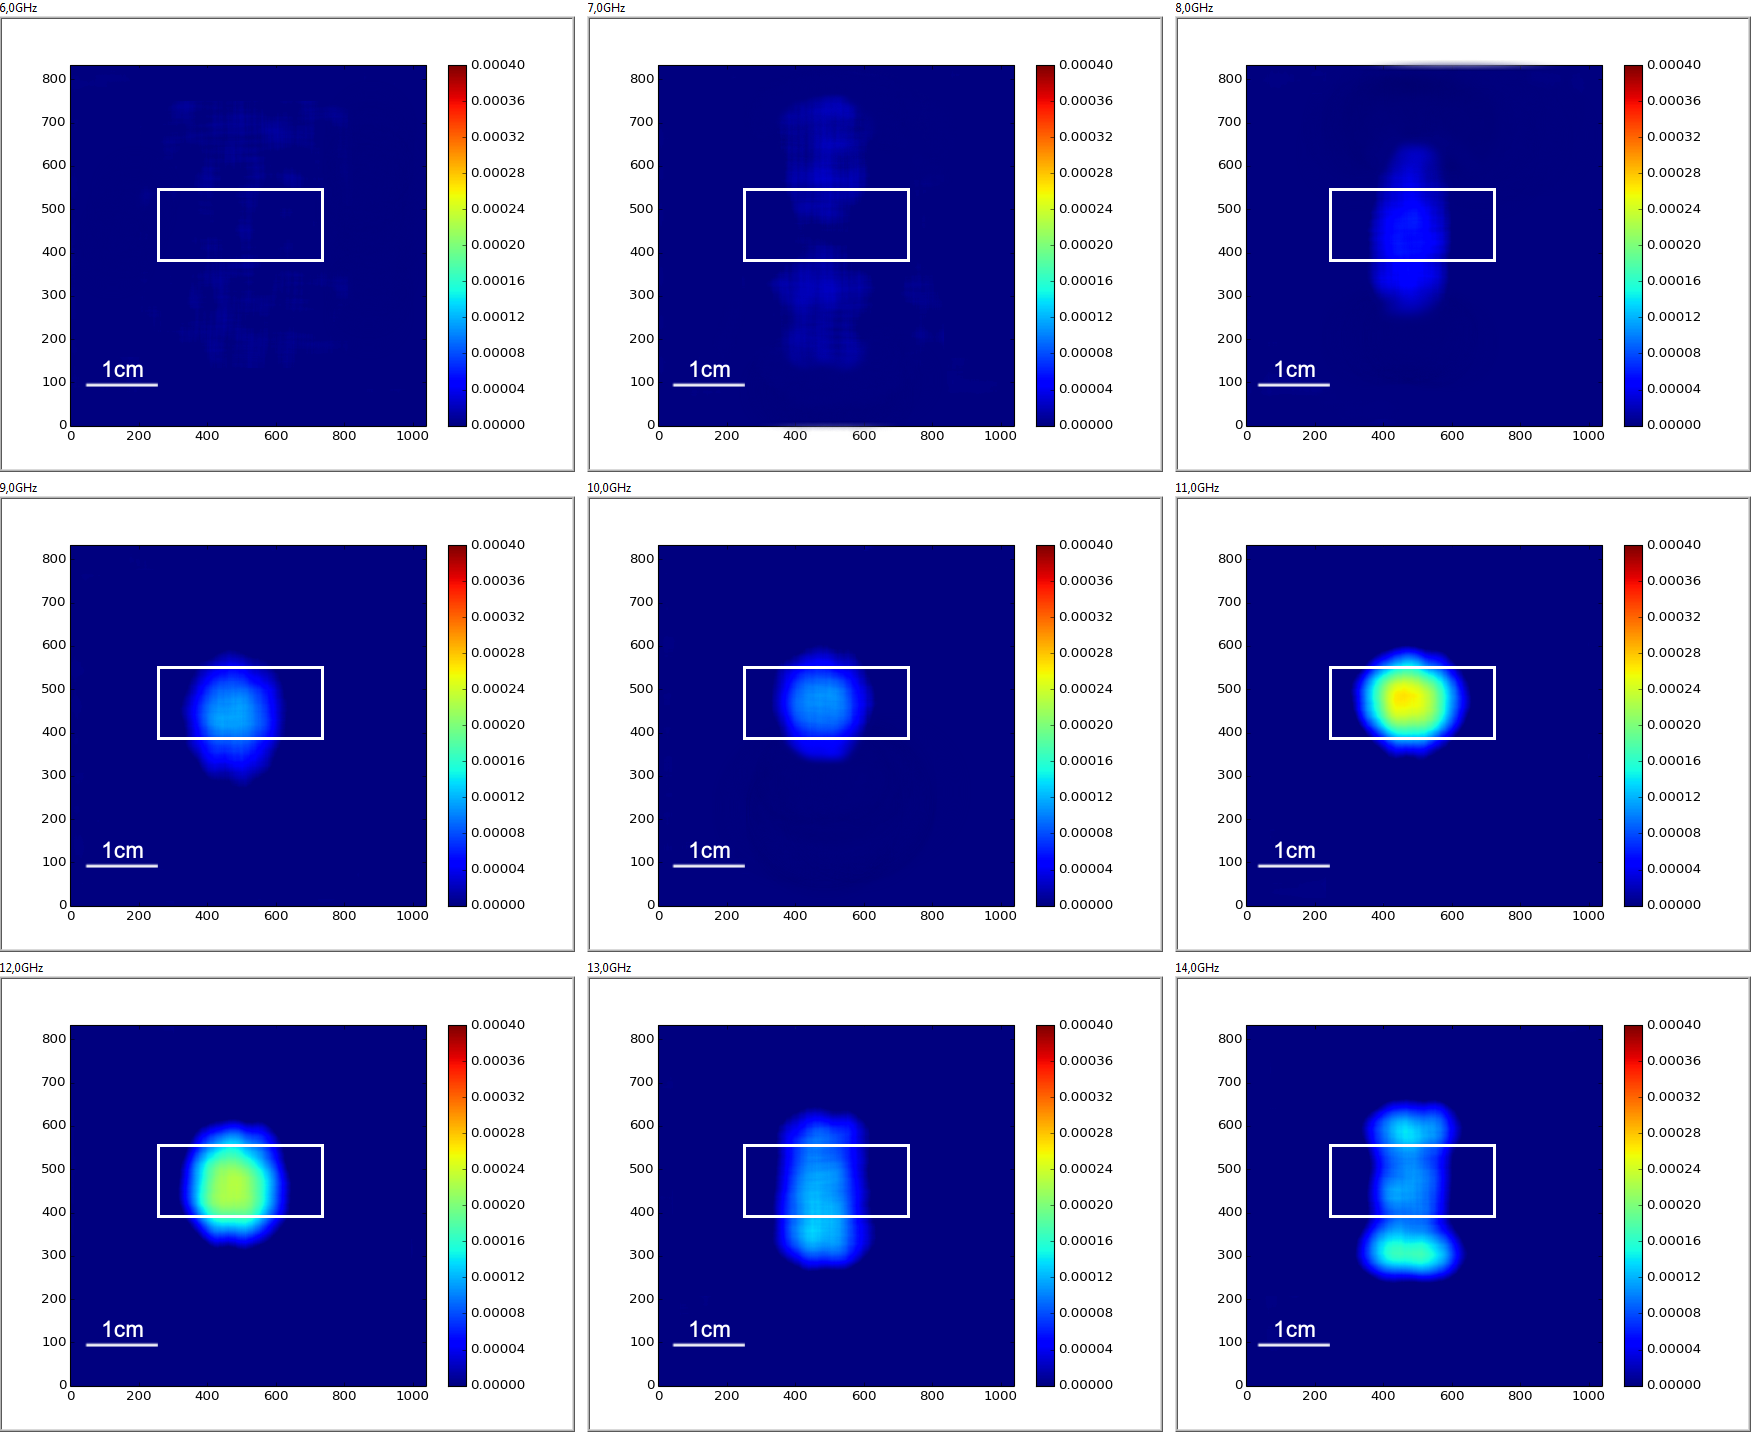
\includegraphics[width=1.0\linewidth]{data/experiment-results/free field of antenna, 6-14ghz, 0dbm generator output, distance 5mm.png}
    \caption{0 dBm հզորությամբ գեներացված էլեկտրամագնիսական ալիքների դեպքում մագնիսական դաշտի ինտենսիվությունները յուրաքանչյուր հաճախության ալիքների համար։ Պատկերները ցույց են տված ըստ հաճախության աճման՝ ձախից աջ, վերևից ներքև հաջորդականությամբ։}
    \label{fig:0dBm-diagram}
\end{adjustwidth}
\end{figure}
Յուրաքանչյուր պատկերներում նաև ցույց է տրված ուղղանկյուն ալիքատարի կտրվածքի դիրքը և չափը։
\begin{figure}
    \begin{adjustwidth}{-1.5cm}{}
    \centering
     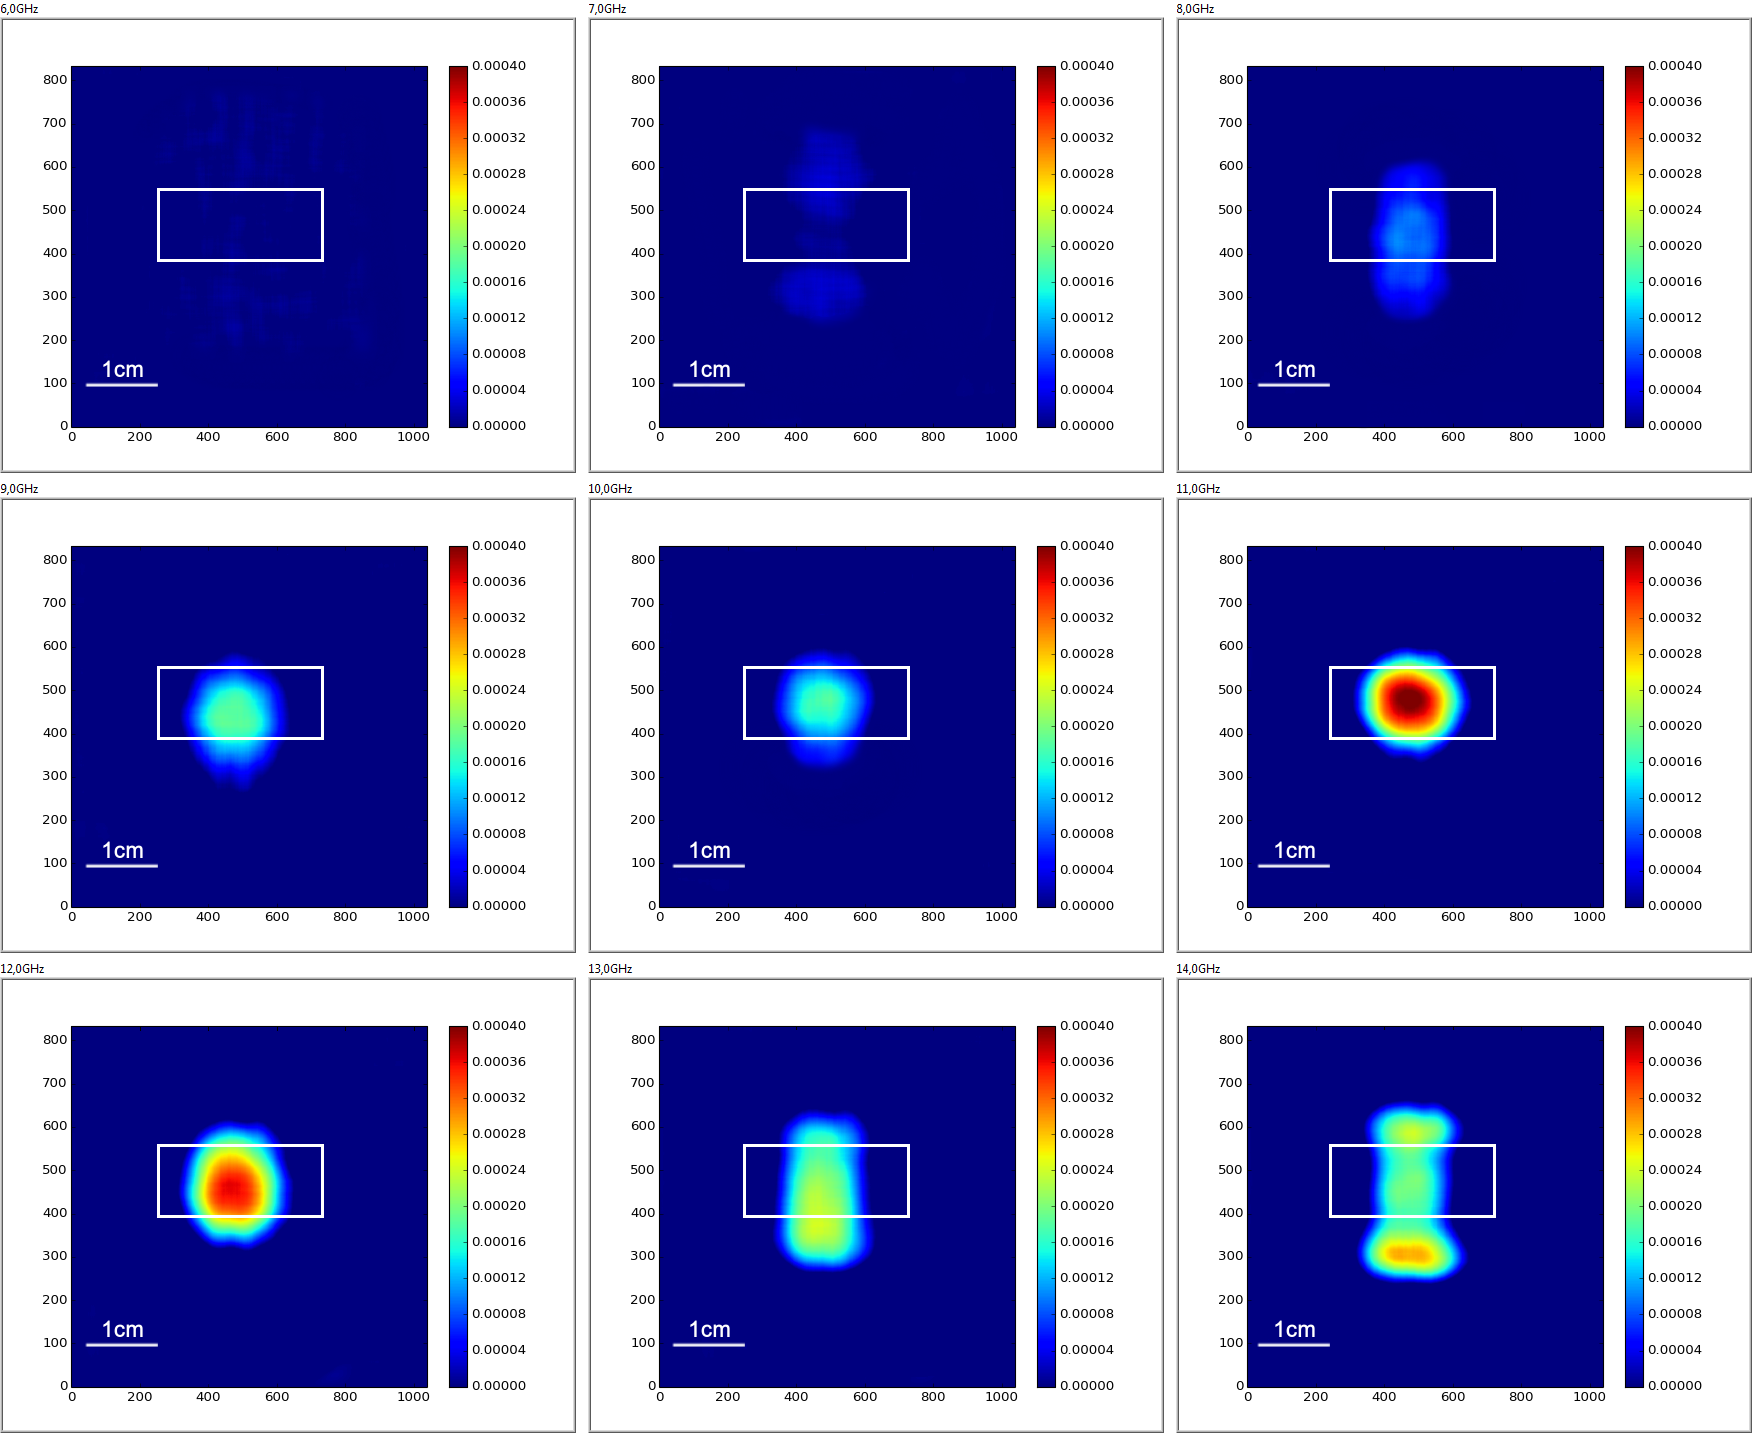
\includegraphics[width=1.0\textwidth]{data/experiment-results/free field of antenna, 6-14ghz, 3dbm generator output, distance 5mm.png}
    \caption{3 dBm հզորությամբ գեներացված էլեկտրամագնիսական ալիքների դեպքում մագնիսական դաշտի ինտենսիվությունները յուրաքանչյուր հաճախության ալիքների համար։ Պատկերները ցույց են տված ըստ հաճախության աճման՝ ձախից աջ, վերևից ներքև հաջորդականությամբ։}
    \label{fig:3dBm-diagram}
\end{adjustwidth}
\end{figure}

\begin{figure}
    \begin{adjustwidth}{-1.5cm}{}
    \centering
    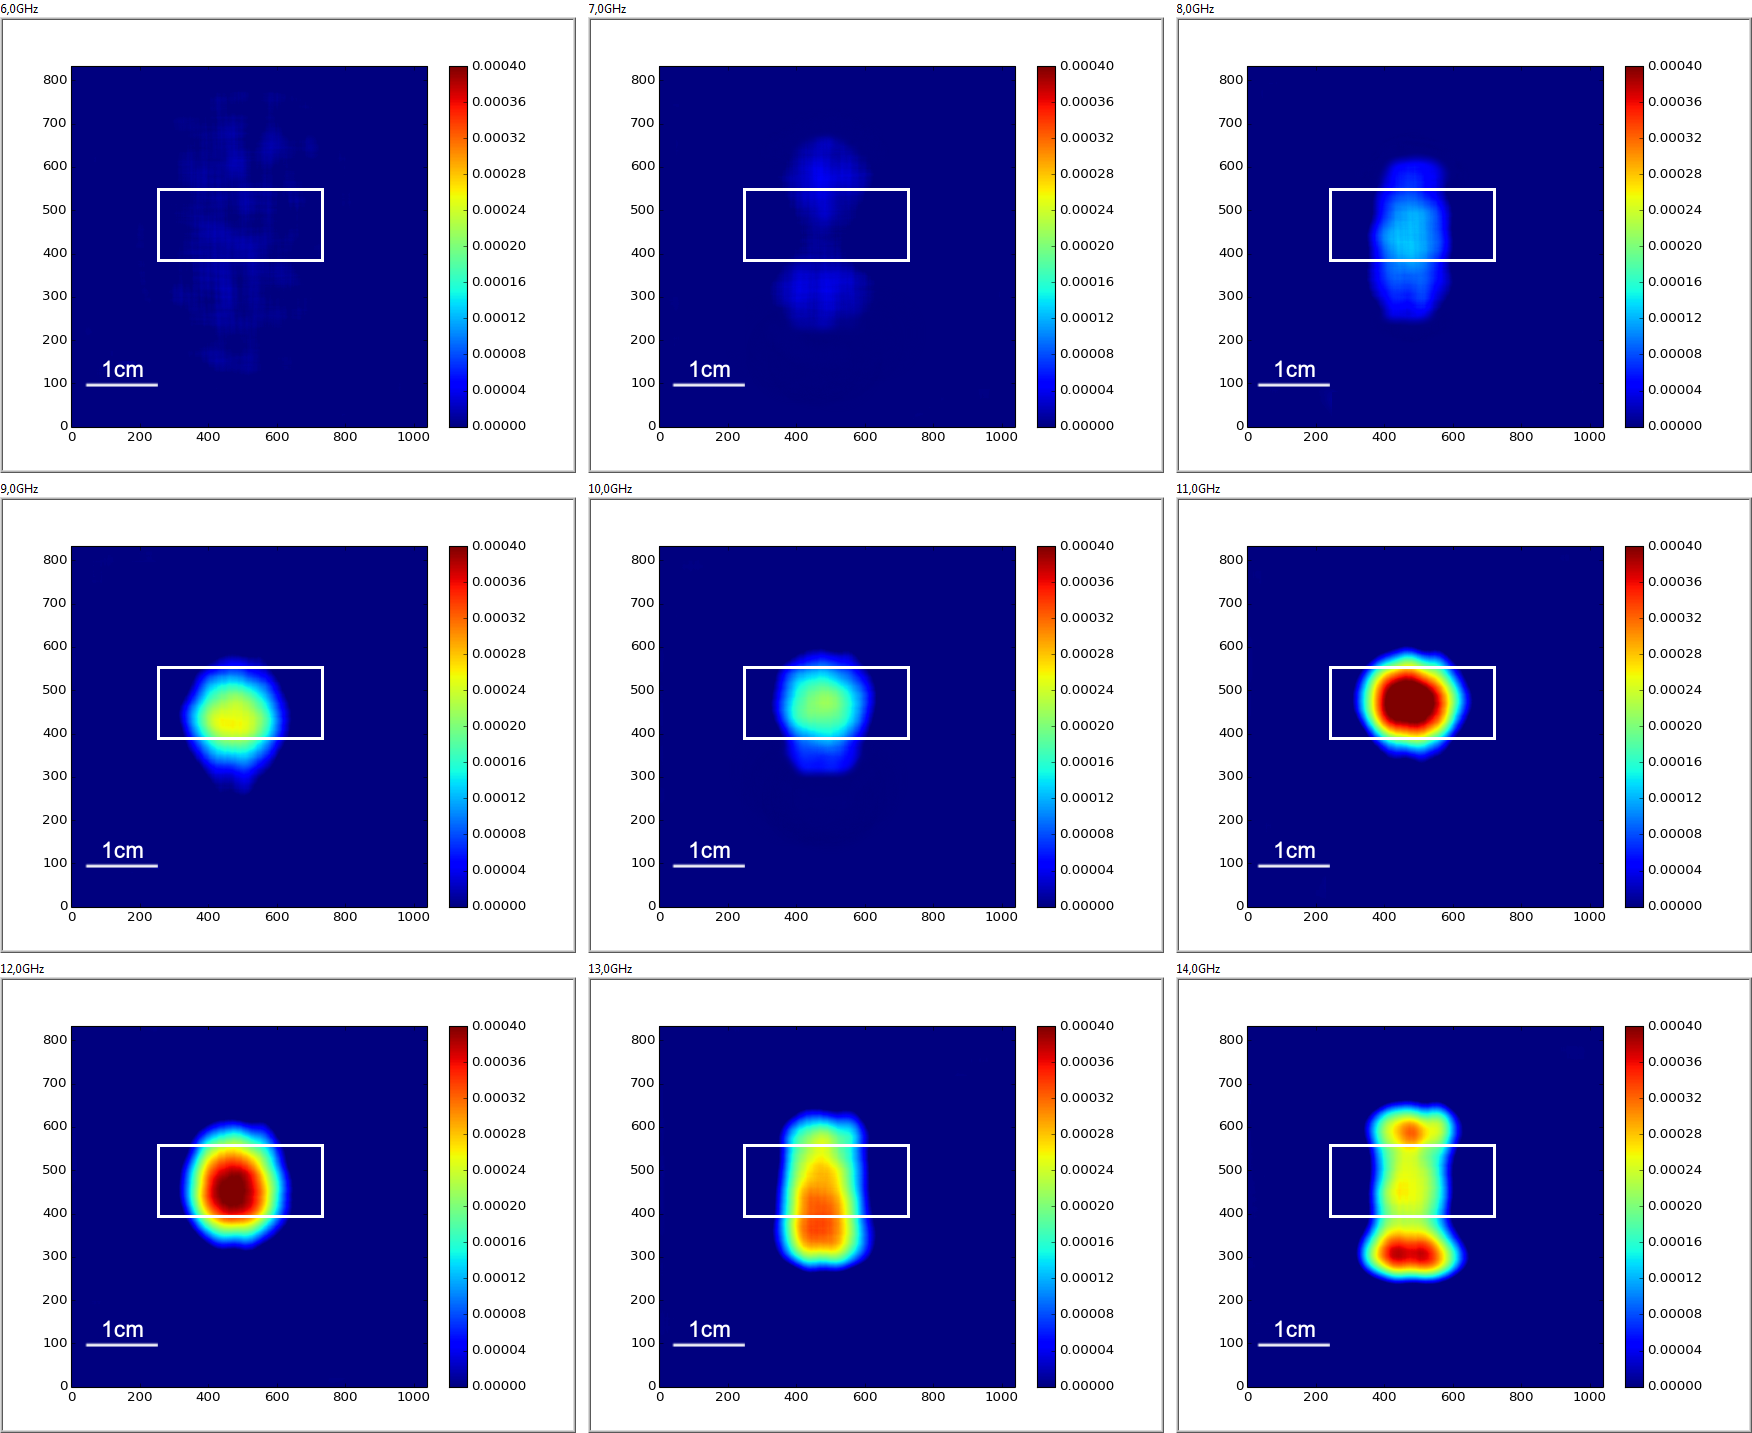
\includegraphics[width=1.0\textwidth]{data/experiment-results/free field of antenna, 6-14ghz, 6dbm generator output, distance 5mm.png}
    \caption{6 dBm հզորությամբ գեներացված էլեկտրամագնիսական ալիքների դեպքում մագնիսական դաշտի ինտենսիվությունները յուրաքանչյուր հաճախության ալիքների համար։ Պատկերները ցույց են տված ըստ հաճախության աճման՝ ձախից աջ, վերևից ներքև հաջորդականությամբ։}
    \label{fig:6dBm-diagram}
\end{adjustwidth}
\end{figure}
Ինչպես տեսնում ենք, հաճախությունը բարձրացնելիս՝ ալիքատարի մագնիսական դաշտի ինտենսիվությունը բարձրանում է և վերաբաշխվում։ Նույն վարքը տեղի է ունենում բոլոր 0, 3 և 6 dBm հզորություններում։ Նկատի առնենք, որ ալիքատարը օգտագործվել է նաև իր աշխատանքային հաճախային տիրույթից դուրս հաճախություններում։ Օրինակ՝ 6, 7, 13 կամ 14 ԳՀց հաճախությամբ ալիքներ են անցկացվել ալիքատարով։ Ինչպես տեսնում ենք նկարներում, ալիքատարի աշխատանքային տիրույթից ցածր հաճախությունների դեպքում մագնիսական դաշտը ունի անկանոն տեսք և ցածր ինտենսիվություն։ Սա պայմանավորված է ալիքատարում ցածր հաճախությամբ էլեկտրամագնիսական ալիքների անդրադարձմամբ։ Բարձր հաճախությունների դեպքում, ինչպես օրինակ 13 կամ 14 ԳՀց, մագնիսական դաշտը կրկին կրում է անկանոն տեսք, ինչը պայմանավորված է ալիքատարում ալիքների անդրադարձումների, ինտերֆերենցիաների և այլ տեսակի շեղումների առկայությամբ։ Այս ամենին համեմատ, ալիքատարի աշխատանքային տիրույթում անցկացված ալիքների մագնիսական դաշտի ինտնեսիվությունը հաճախության բարձրացման հետ աճում է։

Նկ․ \ref{fig:Int_vs_Freq_0_3_6_dBm}֊ում ցույց է տրված վերը նշված հզորությունների դեպքում ալիքատարից ճառագայթված մագնիսական դաշտի միջին ինտենսիվության կախումը [6, 14] ԳՀց միջակայքում ալիքի հաճախությունից։
\begin{figure}
    \centering
    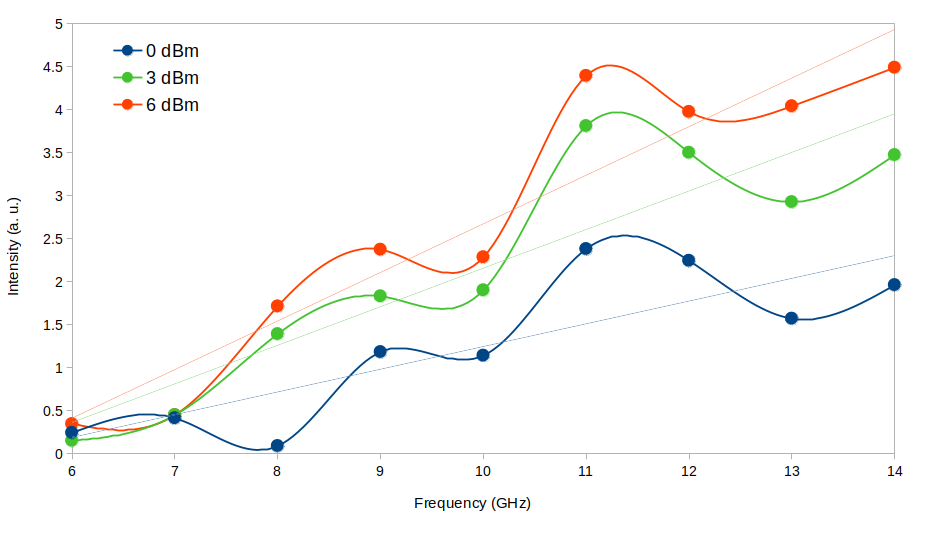
\includegraphics[width=1.0\textwidth]{data/experiment-results/free_field_of_antenna_6-14GHz_0-6dBm_generator_output_distance_5mm.png}
    \caption{Ալիքատարի մագնիսական դաշտի միջին ինտենսիվության կախումը հաճախությունից՝ բոլոր երեք հզորություններով էլեկտրամագնիսական ալիքների գեներացումների դեպքում։}
    \label{fig:Int_vs_Freq_0_3_6_dBm}
\end{figure}
Փորձը ցույց է տալիս, որ մագնիսական դաշտի միջին ինտենսիվությունը [6-14] ԳՀց միջակայքում ալիքի հաճախության բարձրացման հետ աճում է գծայինին մոտ օրենքով։

\renewcommand{\bibname}{Գրականություն}
\begin{thebibliography}{9}

\bibitem{yue2012nanoscalethermal}
Yue, Y. \& Wang, X. Nanoscale thermal probing. Nano Reviews. 3, 11586 (2012).

\bibitem{xie1990picosecond}
Xie, X., Simon, J. D. Picosecond circular dichroism spectroscopy: a Jones matrix
analysis. J. Opt. Soc. Am. B 7, 1673 (1990).

\bibitem{arakelyan2016teoim}
H. Lee, S. Arakelyan, B. Friedman, K. Lee, Temperature and microwave near field imaging by thermo-elastic optical indicator microscopy, Sci. Rep. 6, 39696 (2016).

\bibitem{barron2011thermalstress}
 Barron R. F., Barron B. R. Design for Thermal Stresses. Ch. 6 (Wiley, 2011).

 \bibitem{chen2013itofabcrication}
 Chen Z, Li W, Li R, Zhang Y, Xu G, Cheng H. Fabrication of highly transparent and conductive indium-tin oxide thin films with a high figure of merit via solution processing. Langmuir. 2013 Nov 12;29(45):13836-42. doi: 10.1021/la4033282. Epub 2013 Oct 28. PMID: 24117323.
\end{thebibliography}

\addcontentsline{toc}{section}{Գրականություն}

   
\end{document}
